\documentclass[pre,reprint,superscriptaddress]{revtex4-2}
%\documentclass[utf8, babel, sor, jor, amsmath, amssymb, %reprint]{elsarticle} %удалить перед отправкой

\usepackage{graphicx}
\usepackage[version=4]{mhchem}
\usepackage{amssymb}
\usepackage{bm}% bold math
\usepackage{epsfig}
\usepackage{graphicx}
\usepackage{amsmath}
\usepackage{color}
\usepackage{longtable}
\usepackage{inputenc}
\usepackage{tabularx}
\usepackage{graphicx}% Include figure files
\usepackage{dcolumn}% Align table columns on decimal point
\usepackage{bm}% bold math
%\usepackage[mathlines]{lineno}% Enable numbering of text and display math
%\linenumbers\relax % Commence numbering lines

\begin{document}

\title[Sample title]{Apamea Spin Ice}% Force line breaks with \\
\thanks{Footnote to title of article.}
%\title{Thermodynamics and ground states of Apamea dipolar spin ice}% to be changed


\author{Yuriy Shevchenko}
\email{shevchenko.yuriy.a@gmail.com}
\affiliation{Far Eastern Federal University, Vladivostok, 
	Russian Federation}
\affiliation{Institute of Applied Mathematics, Far Eastern Branch, 
	Russian Academy of Science, Vladivostok, Russian Federation}
\author{Vladislav Strongin}
\affiliation{Far Eastern Federal University, Vladivostok, 
	Russian Federation}
\affiliation{Institute of Applied Mathematics, Far Eastern Branch, 
	Russian Academy of Science, Vladivostok, Russian Federation}
\author{Ivan Trefilov}
\affiliation{Far Eastern Federal University, Vladivostok, 
	Russian Federation}
\affiliation{Institute of Applied Mathematics, Far Eastern Branch, 
	Russian Academy of Science, Vladivostok, Russian Federation}
\author{Eliza Lobanova}
\affiliation{Far Eastern Federal University, Vladivostok, 
	Russian Federation}
\affiliation{Institute of Applied Mathematics, Far Eastern Branch, 
	Russian Academy of Science, Vladivostok, Russian Federation}
\author{Pavel Ovchinnikov}
\affiliation{Far Eastern Federal University, Vladivostok, 
	Russian Federation}
\affiliation{Institute of Applied Mathematics, Far Eastern Branch, 
	Russian Academy of Science, Vladivostok, Russian Federation}
\author{Konstantin Nefedev}
\author{Nikita Ternovoi}
\email{nefedev.kv@dvfu.ru}
\affiliation{Far Eastern Federal University, Vladivostok, 
	Russian Federation}
\affiliation{Institute of Applied Mathematics, Far Eastern Branch, 
	Russian Academy of Science, Vladivostok, Russian Federation}

\date{\today}% It is always \today, today,
             %  but any date may be explicitly specified

\begin{abstract}
An article usually includes an abstract, a concise summary of the work
covered at length in the main body of the article. It is used for
secondary publications and for information retrieval purposes. 
%
\end{abstract}

\keywords{Suggested keywords}%Use showkeys class option if keyword
                              %display desired
\maketitle

\begin{quotation}
The ``lead paragraph'' is encapsulated with the \LaTeX\ 
\verb+quotation+ environment and is formatted as a single paragraph before the first section heading. 
(The \verb+quotation+ environment reverts to its usual meaning after the first sectioning command.) 
Note that numbered references are allowed in the lead paragraph.
%
The lead paragraph will only be found in an article being prepared for the journal \textit{Chaos}.
\end{quotation}

\section{Introduction}
Plan of the paper (remove later):\\
fig 1 - Description of the lattice and vertex types\\
fig 2 - ground state (long range and short-range)\\
fig 3 - to compare the GS with experiment in term of vertex population\\
fig 4, 5 -  energy and heating. crossover or phase transition?.
Look at (https://www.nature.com/articles/s41567-022-01555-6) fig. 5. Try to caluclate the entropy like there.\\
%fig 6,7 - frustrated spins, its activity and compare with simulations\\
fig 6.1,... - Magnetic structure factor (for different temperatures, for different points on heat capacity)\\ (https://www.science.org/doi/10.1126/sciadv.aav6380)
fig 6.2 - dynamic structure factor \\
fig 7  - to calculate the line of instability or Almeida-Thaulesa line, HT -diagramm)\\ 
fig 8 Heat capacity temperature dependence (add points from experiment)\\
fig 9 Distribution of frustration (excitation in the spin ice and paramagnetic)\\
fig 10 To calculate DOS and mark experimental points and gs
 

Artificial spin ice systems, consisting of single-domain nanomagnets that are lithographically defined onto a varity of two-dimensional geometries have emerged in recent years as perfect model systems to directly visualize the consequence of magnetically frustrated interactions with real-space imaging techniques \cite{Skjaervo2020}. Among others, prominent examples feature the direct observation of emergent magnetic monopole dynamics in macroscopically degenerate artificial square ice \cite{Farhan2019}, phase transitions in bridged artificial kagome spin ice \cite{Hofhuis2022,Brunn2021} and the realization of artificial spin glasses~\cite{Saccone2020,Saccone2022}. One of the more fascinating sub-class systems of artificial spin ice has been that of vertex-frustrated systems~\cite{Gilbert2014,Gilbert2015,Saglam2021,Stopfel2018,Saccone2019,Strongina2021,Saccone2023}. Most of these systems are based on the the classical square ice geometry~\cite{Wang2006}, but where selected nanomagnets are removed, resulting in lattices that feature a mixture of four-, three- and two-nanomagnet vertices. As a consequence of geometrical constraints, due to vertex frustration, not all dipolar interactions can be minimized at the same time, most crucially at three-nanomagnet vertices. As a result, these systems feature a non-trivial ground state question and a range of exotic emergent phenomena, starting from emergent ice-rules~\cite{Gilbert2014,Saccone2019} to emergent reduced dimenstionalities~\cite{Gilbert2015}. Among these vertex-frustrated systems, the recently introduced Apamea lattice [see Fig.~\ref{fig:fig1}] represents an interesting case, exhibiting both ergodicity breaking thermodynamics and a non-trivial ground state question~\cite{Saccone2023}.


%{		Эргодическая гипотеза в статистической физике —  средние по времени значения физических величин, равны их средним статистическим значениям.Эргодическая гипотеза, представленная Больцманом в 1887 г., предполагает, что при условии бесконечного времени эксперимента, термодинамическая система будет находятся во всех разрешенных состояниях, причем время нахождения  будет пропорционально энергии и кратности вырождения, быстро приводя средние значения по повторяющимся ансамблям в соответствие со средними значениями с течением времени. Для произвольной физической системы – как классической, так и квантовой – эргодическая гипотеза не доказана. Достаточно строгие доказательства эргодической гипотезы имеются лишь для некоторых простейших физических систем, например идеальных газов, состоящих из большого числа частиц и находящихся в классическом режиме (при высоких температурах и малых концентрациях).		Однако прогнозируется, что будут возникать исключения, поскольку эргодичность имеет тенденцию нарушаться вокруг фазовых переходов, кроссоверов, или в фазе спинового стекла. 	Предполагается, что локальные ограничения в квантовых системах также могут привести к динамике, нарушающей эргодичность15. 	Общая схема измерения эргодичности динамической системы состоит в том, чтобы определить подходящую координату и посмотреть, достаточно ли быстро она рандомизируется с течением времени. В эргодической системе среднее значение координаты по времени эквивалентно среднему значению координаты в пространстве при достаточно большой выборке поведения системы. Метрика стресса28, \varOmega (t), определяется как разница между пространственным средним и средним по времени при наблюдении образца в течение времени t29 (Методы). Эта метрика обычно затухает по степенному закону, \varOmega \left(t\right)\propto {t}^{-z}, и эргодические системы затухают с z = 1, в то время как системы, нарушающие эргодичность, имеют значения z от 1 до 0 из-за к тому, что они попадают в подмножество всех возможных состояний. Мы рассчитываем метрику напряжения нашей системы, рассматривая «пространственное» среднее значение как координаты вращения Изинга для каждого кадра, а «временное» среднее значение — это среднее значение координат Изинга по всем последовательно снятым изображениям (Методы). Мы рассчитали метрику напряжения на каждом временном шаге для каждой зарегистрированной температуры (рис. 4а), чтобы извлечь мощность затухания z с помощью обычной линейной регрессии по методу наименьших квадратов величины \log \left(\varOmega \left(t\right)\right ) в зависимости от журнала времени log (t), получая стандартную ошибку подбора параметров процесса, и строить график ее поведения в зависимости от температуры (рис. 4б). Значение z колеблется около нуля как при высоких, так и при низких температурах, поскольку система, по-видимому, отвергает релаксацию за пределами определенных областей фазового пространства. То есть система быстро восстанавливается после кратковременных колебаний, которые проявляются как резкий рост показателя стресса. Низкотемпературное замерзание является обычным явлением для искусственного спинового льда, поскольку скорость колебаний пермаллоя уменьшается, но сохранение высокотемпературных систем в одном и том же бассейне является своеобразным. Поскольку система хорошо отожжена после более чем 4 недель при температуре 300 К, она, вероятно, находится глубоко внутри зоны притяжения и ограничена в возможностях выхода из нее.  }

The ground state of the spin ice system, as was shown in ~\cite{Makarova2021}, can be composed of ground states of subsystems. In real systems, ground state clusters can be observed, but the internal disorder associated with fabrication and the blocking temperature of nanomagnets can significantly slow down and impede relaxation to the long-range ordered ground state ~\cite{Farhan2013, Hofhuis2020, Farhan2020}.

In spin ices, due to frustration (localized violation of the ice rule~\cite{Bramwell2001}), virtual magnetic monopoles arise, which are not "real" magnetic charges but are topological defects in the spin configuration~\cite{Castelnovo2008}. Previously, monopoles in spin ice were observed as lattice vertices with three adjacent particles~\cite{Mengotti2011} (further - triangular vertices) and four adjacent particles~\cite{Farhan2019} (further - square vertices). It also makes sense to call vertices with two adjacent particles angular and linear.
% The first direct observation of spontaneous formation and separation of magnetically charged defects, or type III vertices, in thermally active artificial square ice was obtained in 2013 . Such defects in artificial square ice, sometimes referred to as monopoles. Important for determining the behavior of monopoles are the background magnetic configuration and geometry of the artificial spin ice, which can be modified by introducing defects into the lattice. 
% In artificial square ice, string tension can be used to produce spontaneous magnetic currents by stretching the bound monopoles with an applied magnetic field and releasing the field to free them.
% Characterization of the resulting magnetic monopoles in real space in the framework of Debye-Hückel theory and visual evidence that these topological defects act as a plasma of Coulomb-type magnetic charges. In contrast to vertex defects in purely two-dimensional artificial square ice, magnetic monopoles can freely evolve in vacuum without divergence, a magnetic Coulomb phase characterized by pinch-point singularities in magnetic structural factors.

In the magnetic-structural factor, the intensity peaks are determined by the lattice geometry to a much greater extent than the temperature \cite{Farhan2019, Farhan2020}. In this paper, we establish this connection. The magnetic-structural factor shows the intensity distribution of neutrons passing through the material, incident perpendicular to the plane on which the spin ice nano-islands are located.

Below we analyze the violation of the ice rule for different types of Apamea lattice vertices (observed in this work at temperatures in the range from 240 K to 290 K) and thus establish that it is the energy distribution of triangular vertices that differs most strongly from the distribution in the ground state. It is expected to see in the magnetic structure factor the intensity peaks determined by the lattice geometry to a much greater extent than by the temperature \cite{Farhan2019, Farhan2020}. The magnetic-structural factor shows the intensity distribution of neutrons passing through the material, incident perpendicular to the plane on which the spin ice nano-islands are located.


\begin{figure}
  \includegraphics[width=\linewidth]{figure_1.jpg}
  \caption{\label{fig:fig1}Apamea spin ice. (a) Scanning electron microscopy image of the Apamea lattice consisting of nanomagnets with lengths L = 360 nm, width W = 120 nm, and thickness d = 2.6 nm with a lattice parameter a = 500 nm. The yellow scale bar indicates a length of 600 nm. (b) XMCD image of low-energy moment configuration recorded after thermal annealing. While ground state domains emerge, we see sporadic clockwise and anti-clockwise moment loops forming on the irregular hexagonal plaquettes. (c) Vertex types at two-, three-, and four-nanomagnet vertices listed with increasing dipolar energy. For example, the order is from 1 through 4, A through B, etc. Magnetic charges at each vertex, Q, are listed in terms of multiples of the dipole’s fundamental magnetic charge q. Positive Q values are depicted as red and negative values are blue. }
\end{figure}

\section{Ground state candidate}

In Figure ~\ref{fig:fig_gs}, a configuration that is a candidate for the ground state is depicted. This configuration consists of two sublattices alternating in a checkerboard pattern. The particles that differ between the sublattices are highlighted in a different color. All vertices satisfy the ice rules. The figure~\ref{fig:fig_gs_e} for this candidate reflects that only the linear and square vertices are at the minimum.

\begin{figure}
        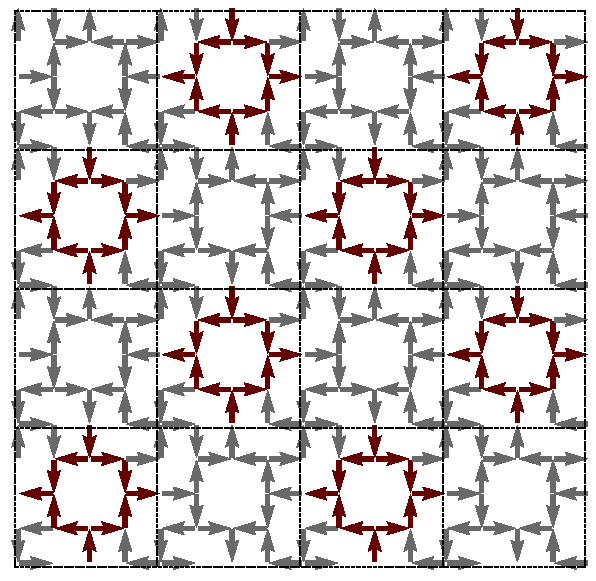
\includegraphics[width=\linewidth]{4x4GS_candidate.pdf}         \caption{\label{fig:fig_gs}GS candidate}
\end{figure}
\begin{figure}
        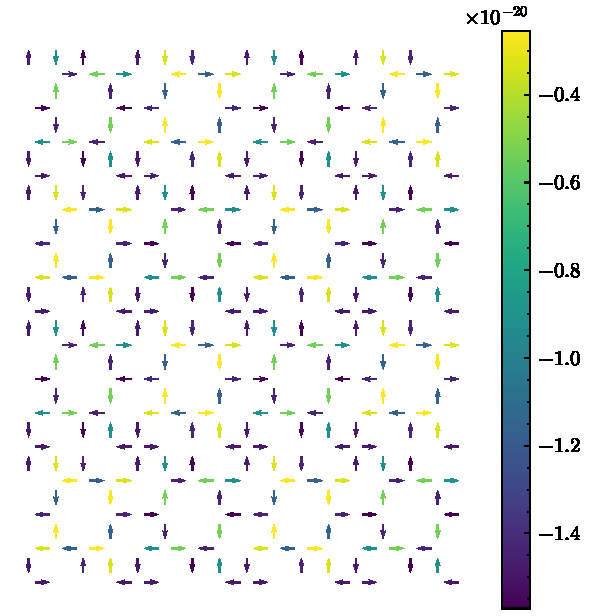
\includegraphics[width=\linewidth]{figs/4x4Cells_energy.pdf}         \caption{\label{fig:fig_gs_e}Energy per spin in GS candidate}
\end{figure}

\section{Vertex population}

In our study of vertex populations, vertices are defined as lattice nodes located at the intersections of edges. Within the examined lattice, we identified two-, three-, and four-particle vertices. Experimental XMCD images revealed that for two-particle vertices, types a and alpha predominated, although the occurrence of types b and beta increased with rising temperature. For three-particle vertices, type C was entirely absent, with type A appearing in approximately 60\% of cases and type B in 40\%. For four-particle vertices, types III and IV were rare, type II appeared in less than 10\% of cases, and type I was almost always present. When investigating the ground state candidate, we found that two-particle vertices exclusively exhibited types a and alpha, with the higher energy types b and beta absent. For three-particle vertices, type C was not observed, type A occurred in about 75\% of cases, and type B in 25\%. Four-particle vertices showed no presence of types II, III, and IV, with type I, the lowest energy configuration, being the only one observed. In the figure~\ref{fig:fig_vertex} we have shown how the experimental data relate to the theoretical modeling.

\begin{figure}
        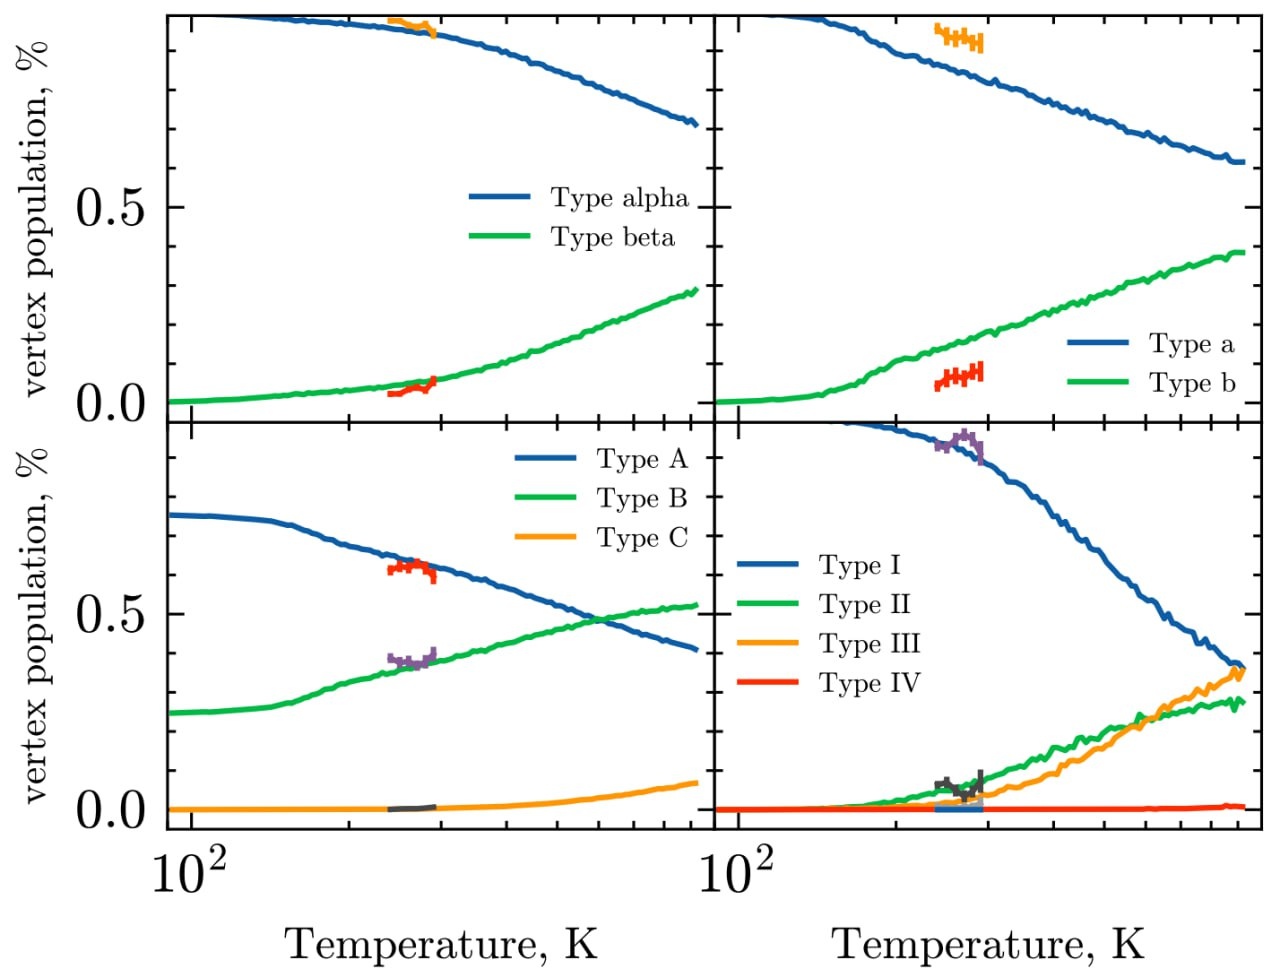
\includegraphics[width=\linewidth]{figs/vertex_population.jpg}         \caption{\label{fig:fig_vertex}Vertex population. The points for which there is no entry in the legend are experimental (averaging over 100 XMCD images for each of the five temperatures represented in the range from 240K to 290K). The rest are calculated using the Metropolis algorithm}
\end{figure}

\section{Magnetic structure factor}

Magnetic structure factor is calculated as:
\begin{equation}
  I(\vec{q}) = \frac{1}{N} \sum^N_{i=1} \sum^N_{j=1} \vec{S}_i^\perp \cdot \vec{S}_j^\perp \exp (i \vec{q} \cdot \vec{r}_{i,j}),
\end{equation}
where $\vec{S}_i^\perp = \vec{S}_i - (\hat{q} \cdot \vec{S}_i ) \hat{q}$ is the component of the spin vector of each island, $\vec{S}_i$, perpendicular to the reciprocal space vector $\vec{q}$, and $\hat{q} = \vec{q} / |\vec{q}|$ \cite{Farhan2019}. 

The Dynamic structure factor is designed to show time-dependent fluctuations of spins. It is defined as:
\begin{equation}
	\mathcal{S} (\vec{q},\omega) = \frac{1}{2 \pi} \int_{-\infty}^{\infty}  I(\vec \exp (iq \cdot r_{i,j}),
\end{equation}

The intensity is proportional to the correlation of the magnetic moments of parallel particles of the system in projection to the direction of the radius-vector of the considered distribution point. Since our material is antiferromagnetic, the correlated directions of magnetic moments will most often occur along those directions along which there are more triangular vertices.



\begin{figure}[t]
	a.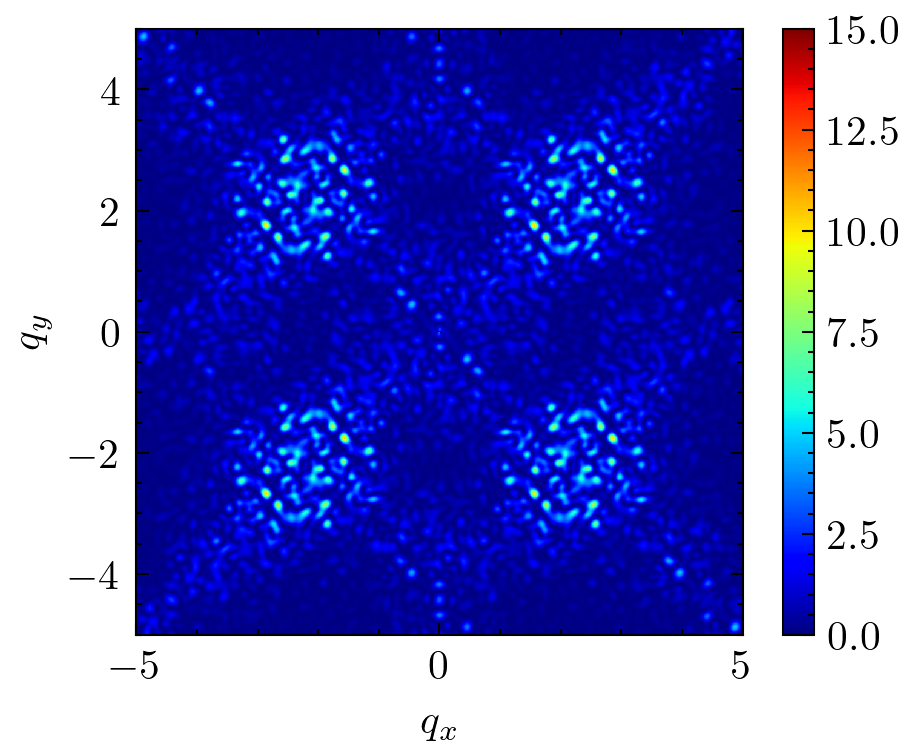
\includegraphics[width=0.45\linewidth]{figs/msf_experiment_240K.png}  
	b.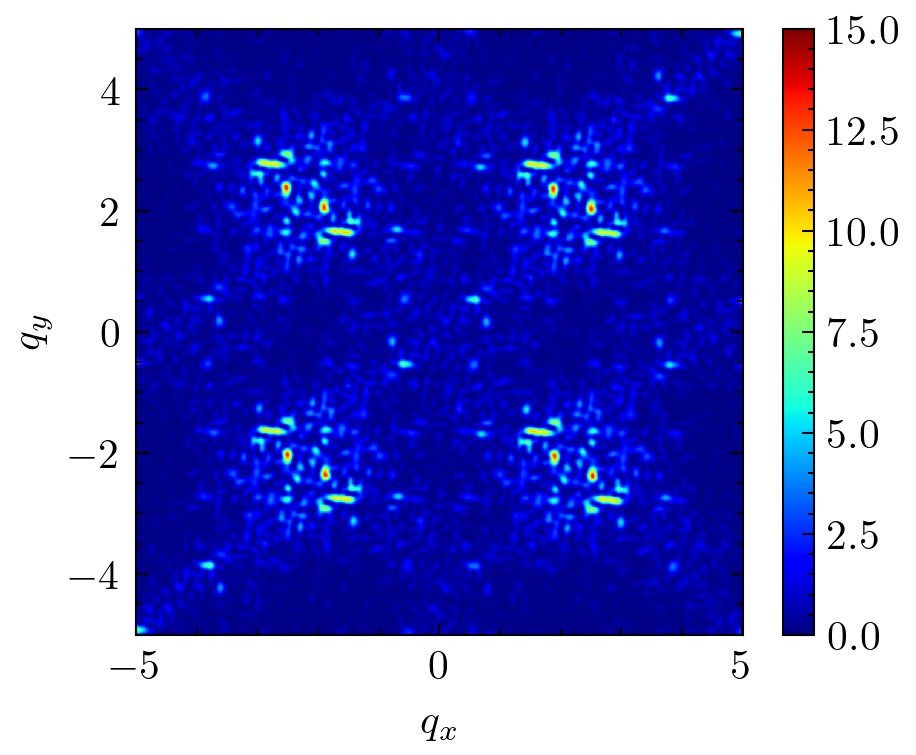
\includegraphics[width=0.45\linewidth]{figs/msf_experiment_250K.png} \\  
	c.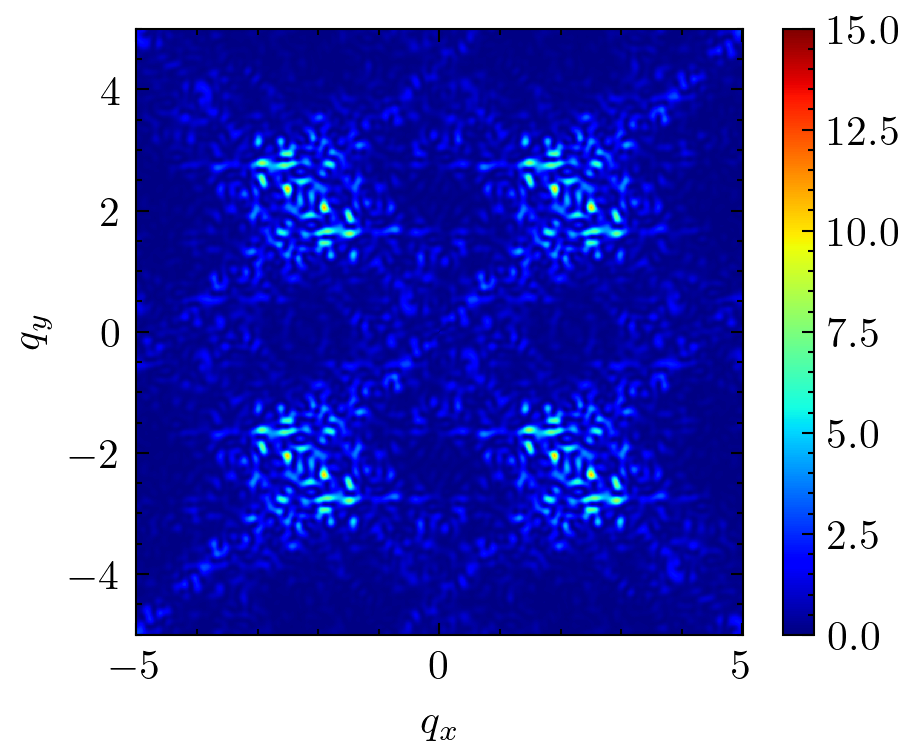
\includegraphics[width=0.45\linewidth]{figs/msf_experiment_260K.png}  
	b.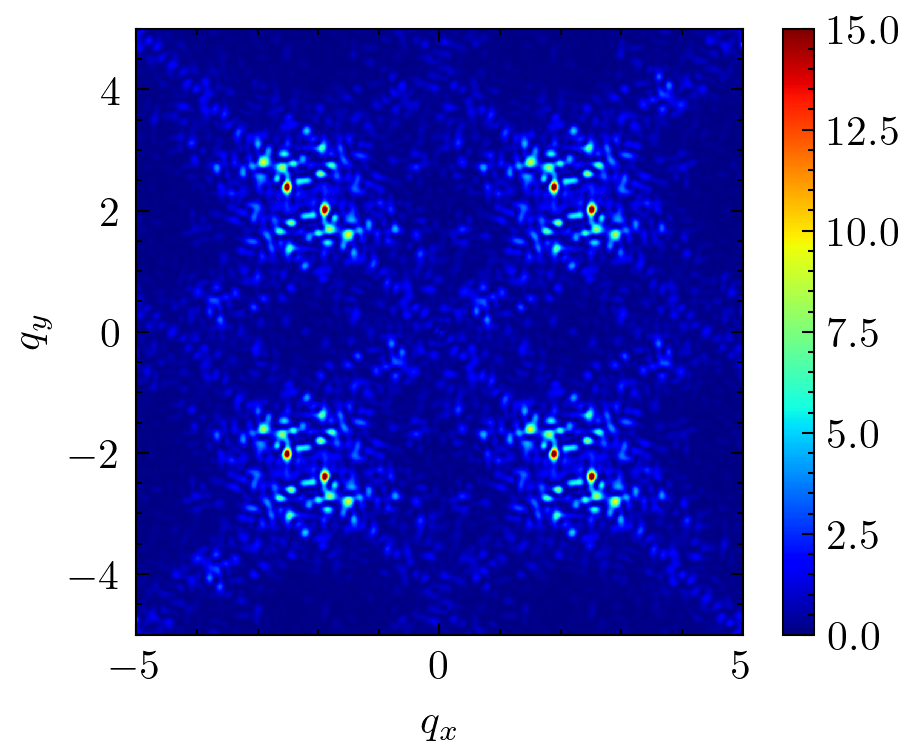
\includegraphics[width=0.45\linewidth]{figs/msf_experiment_270K.png} \\ 
	e.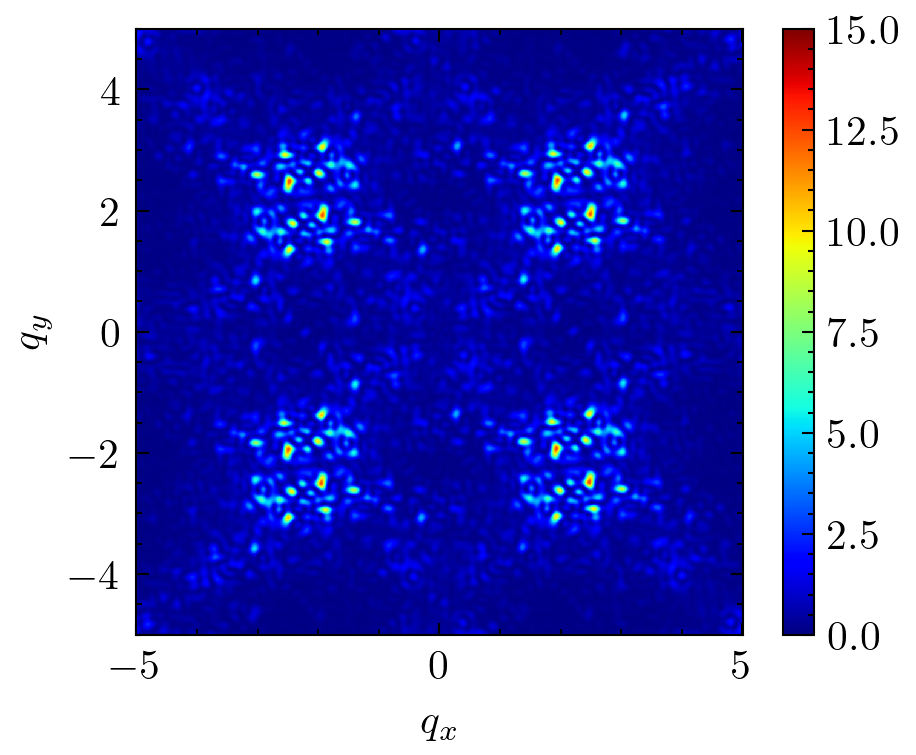
\includegraphics[width=0.45\linewidth]{figs/msf_experiment_280K.png}  
	f.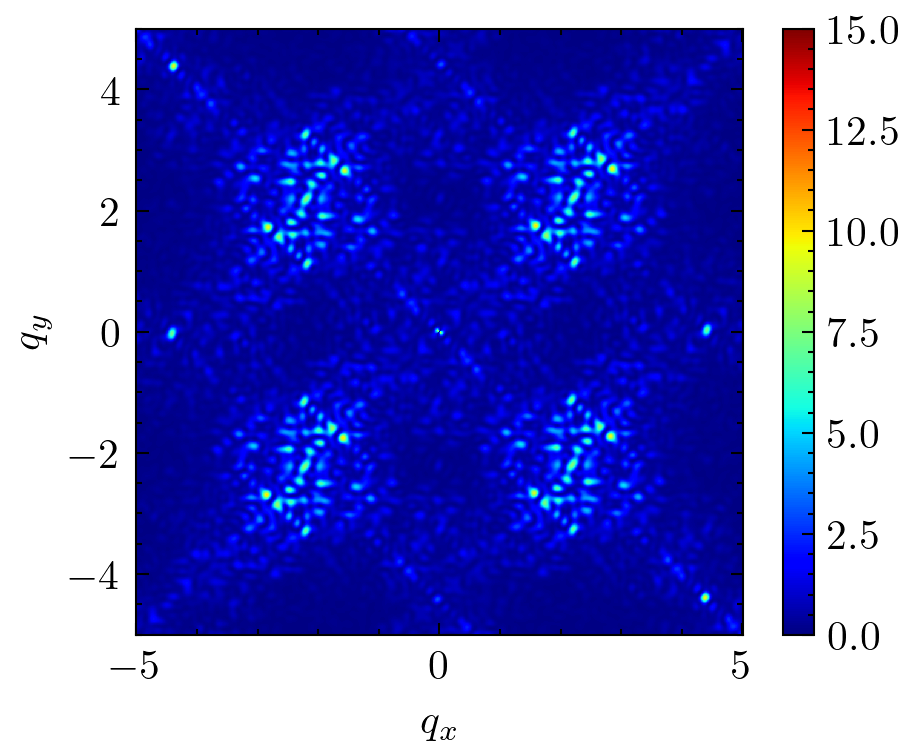
\includegraphics[width=0.45\linewidth]{figs/msf_experiment_290K.png} \\  
	g.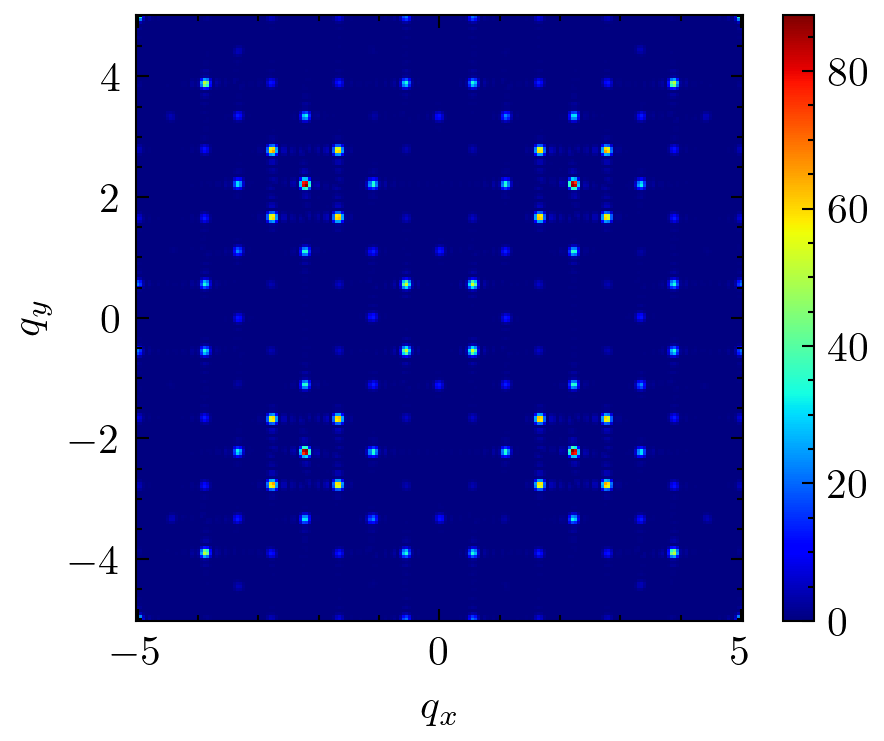
\includegraphics[width=0.45\linewidth]{figs/msf_mc_gs.png} 
	h.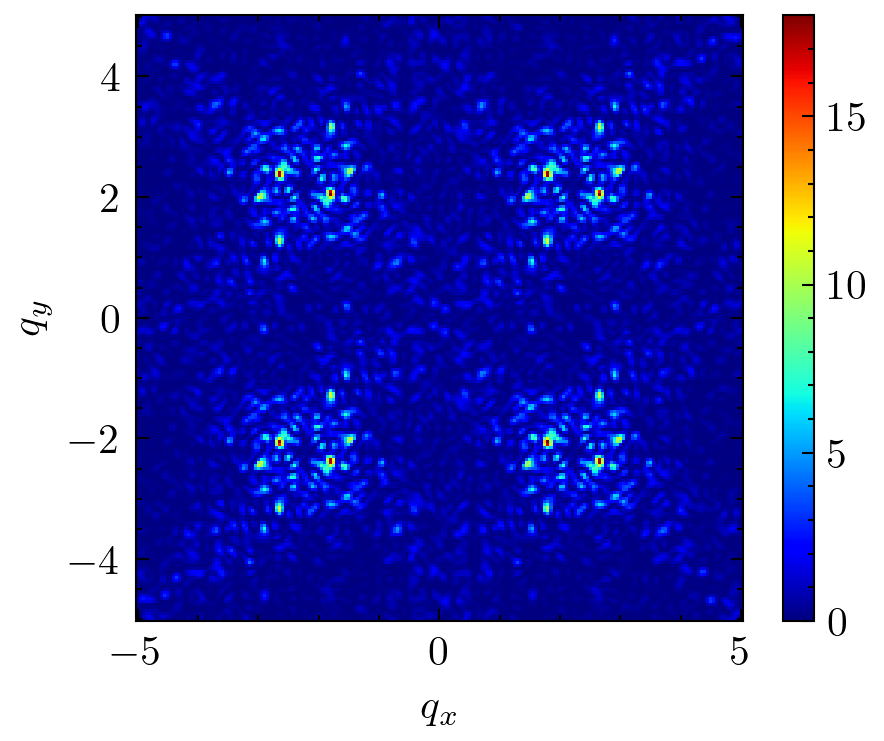
\includegraphics[width=0.45\linewidth]{figs/msf_mc_240K.png} 
	\caption{\label{MSF} Magnetic structure factor 
		(a-f) from the experiment averaged by 100 scans at 240K (a), 250K (b), 260K (c), 
		270K (d), 280K (e), 290K (f)
		(g) Ground-state configuration, (h) MC calculations at 240K}
\end{figure}

\section{Conclusions}
Having plotted the populations for the observed temperatures and for the ground state, we found that all vertices, except for triangular vertices, are close to the ground state in their distributions. So the monopoles influencing the magnetic-structural factor are triangular vertices. Since our material is antiferromagnetic, correlated directions of magnetic moments will most often occur along those directions along which more of these vertices are located. 

The populations of vertices (Fig.~\ref{fig:fig_vertex}) observed in the experiment for types a and b indicate that the system is more strongly correlated than we can assume theoretically from the Metropolis modeling based on the Gibbs~\cite{janke2008monte} distribution. These vertices are just as fully correlated in the ground state candidate we found. This result indicates that we have yet to establish a correct energy distribution model for this system.

\begin{acknowledgments}
We wish to acknowledge the support of the author community in using
REV\TeX{}, offering suggestions and encouragement, testing new versions,
\dots.
\end{acknowledgments}

\nocite{*}
\bibliography{aipsamp}% Produces the bibliography via BibTeX.

\end{document}
%
% ****** End of file aipsamp.tex ******
